The stencil communication pattern is a special case of the gather pattern.
The stencil pattern reads multiple elements in memory defined by some specific offset or pattern to a given input.
This offset or pattern defines specific characteristics of a stencil.
Examples of specific stencils are \textbf{2D/3D von Neumann} and \textbf{2D/3D Moore}.
For further figure references in this section, the green cube/square symbolizes the input element of a stencil operation.
\\\\
The 2D \textbf{von Neumann stencil} reads the input, top, bottom, left and right elements relative to the input element in an array.
The number of \textit{N} elements that are read in a von Neumann stencil in each direction is determined by a "\textit{N}-point von Neumann stencil".
This means that for a 5-point 2D von Neumann stencil would in total result in five reads, while a 9-point 2D von Neumann stencil would in total result in 9 reads.
The number of \textit{N} points in a 2D von Neumann stencil can be formalized as $(N\bmod 4)=1\equiv true$.
Examples of different 2D von Neumann stencils are seen in \autoref{fig:2DvonNeu}.
\begin{figure}[ht]
	\centering
	\begin{subfigure}{.33\textwidth}
		\centering
		\fbox{
			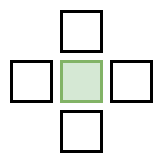
\includegraphics[width=0.4\textwidth]{figs/patterns/5point2DvonNeu.png}
		}
		\caption{5-point 2D von Neumann stencil}
		\label{fig:5p2DNeu}
	\end{subfigure}%
	\begin{subfigure}{.33\textwidth}
		\centering
		\fbox{
			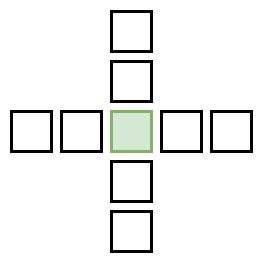
\includegraphics[width=0.6\textwidth]{figs/patterns/9point2DvonNeu.png}
		}
		\caption{9-point 2D von Neumann stencil}
		\label{fig:9p2DNeu}
	\end{subfigure}
	\begin{subfigure}{.33\textwidth}
		\centering
		\fbox{
			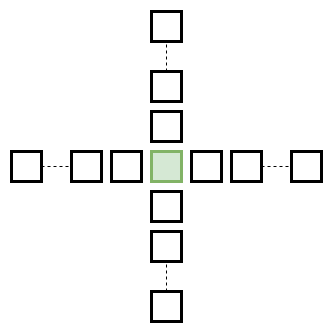
\includegraphics[width=0.6\textwidth]{figs/patterns/Npoint2DvonNeu.png}
		}
		\caption{N-point 2D von Neumann stencil}
		\label{fig:Np2DNeu}
	\end{subfigure}%
	\caption{Different 2D von Neuman stencils}
	\label{fig:2DvonNeu}
\end{figure}
The von Neumann stencils generalizes also to three dimensions.
The main idea is the same as for 2D but with an added dimension.
The number of read data points is thus more compared to the 2D case, and the number of \textit{N} points in a 3D von Neumann stencil can be formalized as $(N\bmod 6)=1\equiv true$.
Examples of 3D von Neumann stencil is seen in \autoref{fig:3DvonNeu}.
\begin{figure}[ht]
	\centering
	\begin{subfigure}{.33\textwidth}
		\centering
		\fbox{
			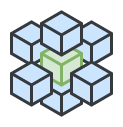
\includegraphics[width=0.4\textwidth]{figs/patterns/7point3DNeu.png}
		}
		\caption{7-point 3D von Neumann stencil}
		\label{fig:7p3DNeu}
	\end{subfigure}%
	\begin{subfigure}{.33\textwidth}
		\centering
		\fbox{
			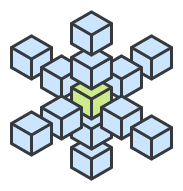
\includegraphics[width=0.6\textwidth]{figs/patterns/13point3DNeu.png}
		}
		\caption{13-point 3D von Neumann stencil}
		\label{fig:13p3DNeu}
	\end{subfigure}
	\begin{subfigure}{.33\textwidth}
		\centering
		\fbox{
			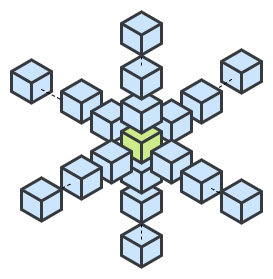
\includegraphics[width=0.6\textwidth]{figs/patterns/Npoint3DNeu.png}
		}
		\caption{N-point 3D von Neumann stencil}
		\label{fig:Np3DNeu}
	\end{subfigure}%
	\caption{Different 3D von Neuman stencils}
	\label{fig:3DvonNeu}
\end{figure}
\\\\
\textbf{Moore stencils} are almost the same as von Neumann stencils, with the exception that  they read \textit{all} neighbors relative to the input element.
This means that the shape of a 2D Moore stencil is a square, while the shape of a 3D Moore stencil is a cube.
The number of \textit{N} points in a 2D Moore stencil can be formalized as $(N\bmod 8)=1\equiv true$ and for the 3D case as $(N\bmod 26)=1\equiv true$.
Examples of Moore stencils is seen in \autoref{fig:Moore}.
\begin{figure}[ht]
	\centering
	\begin{subfigure}{.5\textwidth}
		\centering
		\fbox{
			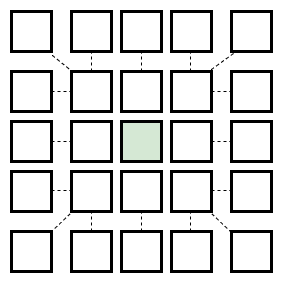
\includegraphics[width=0.4\textwidth]{figs/patterns/Np2dMoore.png}
		}
		\caption{N-point 2D Moore stencil}
		\label{fig:Np2DMoore}
	\end{subfigure}%
	\begin{subfigure}{.5\textwidth}
		\centering
		\fbox{
			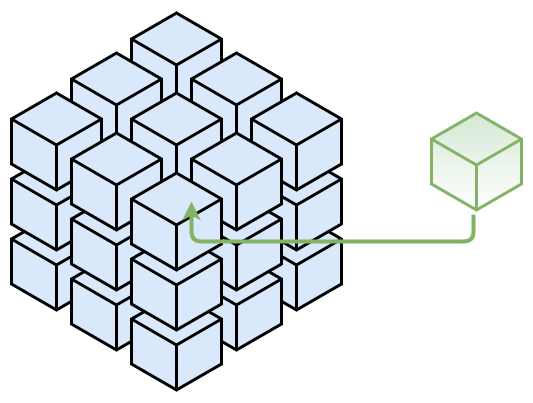
\includegraphics[width=0.6\textwidth]{figs/patterns/Np3dMoore.png}
		}
		\caption{27-point 3D Moore stencil}
		\label{fig:27p3DMoore}
	\end{subfigure}
	\caption{Different types of Moore stencils}
	\label{fig:Moore}
\end{figure}
As can be from \autoref{fig:27p3DMoore} the input element is surrounded by other other elements in the memory grid, and for this reason it is a bit difficult to illustrate that the input element resides inside the cube.
Notice that using 2D Moore stencils is a way of how kernels for image processing are implemented as described in \autoref{sec-gather}.
\\\\
An example of applying a 2D von Neumann stencil to an array of inputs is illustrated in \autoref{fig:2dMooreEx}.
In this case a thread is responsible for applying a single stencil to an input element.
\begin{figure}[ht]
	\centering
	\fbox{
		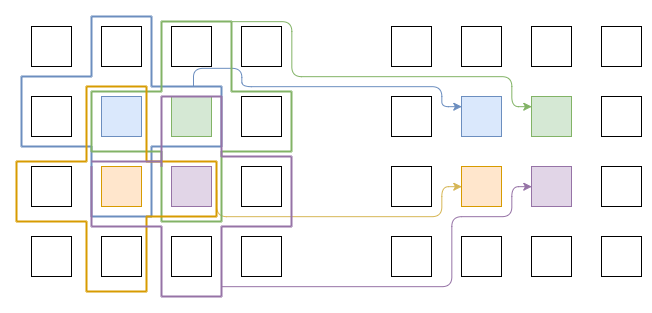
\includegraphics[width=0.6\textwidth]{figs/patterns/2dMooreEx.png}
	}
	\caption{Example of applying 2D Moore stencil}
	\label{fig:2dMooreEx}
\end{figure}
Implementing these stencils are done the same way as with the gather pattern, since stencils are special cases of this pattern.
In the case of applying stencils in parallel exploits a lot of data reuse since multiple threads are overlapping each other.
Implementing the stencil pattern maps very well to CUDA, since it is possible to represent both 2D and 3D structures in CUDA.